\chapter{Introduction}

\par In this paper I propose an application to harness the power of the modern web browser to deliver engaging musicality tutoring based on adaptive learning principles. The application will comprise of various exercises designed to challenge and improve a user's musicality, and keep track of their progress as well as adapt to their strengths and weaknesses in different areas.
\vspace{1em}
\par

\section{Adaptive learning}
As usage of the world wide web has become ubiquitous among citizens of the developed world, web based teaching has grown rapidly to try and modernize learning methods to fit into the 21st century lifestyle. Increasing numbers of companies like Coursera\cite{coursera}, Codeacademy\cite{codeacademy}, Duolingo\cite{duolingo} are providing easily accessible education for anyone with an internet connection and a desire to learn. Codeacademy and Duolingo in particular are notable for their use of rich, highly interactive learning tools which - through requiring the user to have an input into the educational process - establish a feedback system with powerful results\cite{vesselinov2012duolingo}. These companies offer a variety of different programmes the user can study, and each of these is taught through a series of exercises, the results of which are used to track the users progress through the course, and provide statistics on how much they have learned. Duolingo, a website that teaches foreign languages, takes it a step further by introducing adaptive learning methods to recognise the user's proficiency in various areas, information it can then use to tailor-make lessons to fit the user's needs. Duolingo is arguably the best best-known example of an adaptive learning system put into practice. It will therefore often be used for comparison throughout this report, as it has also provided a lot of inspiration for my thinking about the direction my project will take.

\begin{figure}
	\centering
	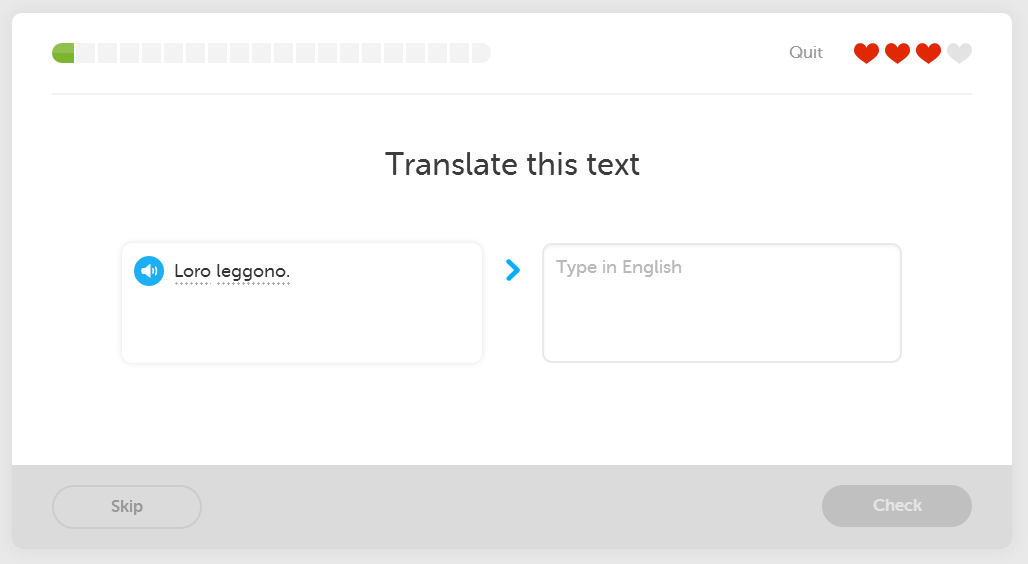
\includegraphics[scale=0.5]{duolingo.png}
	\caption{Duolingo adapts the questions it asks depending on the user's strengths and weaknesses}
\end{figure}

\section{Music teaching on the web}

\vspace{1em}
\par
The web is a great place to train the musical ear, a skill we shall refer to under the term of \bsq{musicality} from hereon in. The rich media options possible on modern day web browsers mean that the input and output of music to a web browser is not only easy to implement, but easy to make user friendly. However, while there are many \bsq{music theory tutors} and \bsq{ear trainers} available, there are no existing adaptive learning solutions. Such a solution would hopefully be invaluable to potential learners as the current best solutions still have no idea who you are and what you've achieved after you leave the page.
\par
In order to teach adaptively we must analyse information about a user's performance, and then change how we teach accordingly. 
There are various ways of measuring musicality, which will be discussed in more detail later, and we will rely on these metrics to adapt the learning experience to fit the user.

\section{Pitch detection}
There are very few examples of pitch detection algorithms running in browser, and the few that there are aren't very useful to a singer\cite{webaudiodemos,audioStretch}. This is because they all try to perform real-time pitch detection where the output is calculated at the same time the user is singing. This is useful for instruments like guitars where when you strike a note, you can be assured it will remain fairly constant in pitch, but the human voice is prone to slight variations in pitch that can cause a real-time algorithm to oscillate around a point, making it hard to gauge what the note you actually sung was. It is with this in mind that I aim to create a meaningful pitch detection algorithm that looks at a 2-3 second audio sample and gives the user accurate pitch data for that period


\section{Achievements}

I have created a web application to train user's intonation using pitch detection and adaptive learning techniques. In doing so, I have created a designed a functional adaptive learning method, as well as a successful pitch detection function for the recognition of sung notes.